\section{Implementarea DVM versiunea 2}

Implementarea simulatorului \gls{dvm} versiunea 2 folosește memoria internă și un fişier aflat în sistemul local de fişiere pentru stocarea și întoarcerea valorilor atributelor modelelor \gls{yang} pe care le expune. Fişierul de configurare conţine valori pentru toţi aceşti parametri și are o structură asemănătoare unui răspuns la operaţia \textit{get} al unui server \gls{netconf}. Această abordare este foarte avantajoasă, din două motive. În primul rând, dacă un dezvoltator de aplicații software \gls{sdn} are nevoie de alte valori pentru orice atribut \gls{yang}, este suficient să modifice acea valoare în fişier și să repornească simulatorul \gls{dvm}, fără sa fie nevoie să cunoască detaliile de implementare sau să recompileze serverul \gls{netconf}. În cel de-al doilea rând, \gls{dvm} poate oferi răspunsuri similare cu un mediator real dacă în fişierul de configurare se va introduce răspunsul \gls{xml} venit de la un astfel de mediator la o operaţie \textit{get}.

Fluxul de lucru pentru operaţiile de aducere a atributelor este ilustrat în Figura \ref{fig:dvm_v02_workflow}.

\begin{figure}[h]
	\centering
	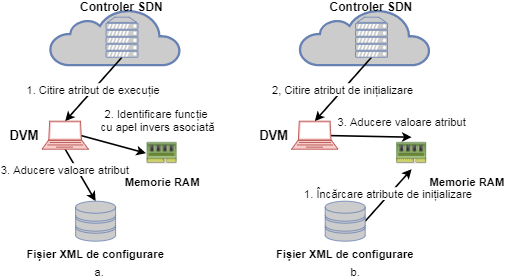
\includegraphics[width=1\textwidth]{dvm_v02_workflow}
	\caption{Fluxul de lucru pentru aducerea atributelor: a) de execuţie; b) de iniţializare \cite{stancu2017enabling}.}
	\label{fig:dvm_v02_workflow}
\end{figure}

Echipamentul de control \gls{sdn} care se conectează la simulatorul \gls{dvm} poate efectua diferite operații asupra parametrilor de execuţie sau de iniţializare.